\documentclass[12pt]{report}
 
\usepackage[utf8]{inputenc}
\usepackage[T1]{fontenc}
\usepackage[german]{babel}
\usepackage{graphicx}
\usepackage{wrapfig}
\usepackage{amsmath}
\usepackage{cleveref}
\usepackage{amsfonts}
\usepackage{amssymb}
\usepackage{tikz}
\usepackage{nicefrac}
\usepackage{mathtools}
\usepackage{cancel}
\usepackage[margin=1in]{geometry}
\usepackage[section]{placeins}

\newcommand{\kq}{\frac{1}{4 \pi \epsilon_0}}
\newcommand{\vabla}{\vec{\nabla}}
\newcommand{\vepsilon}{\varepsilon}
\newcommand{\vphi}{\varphi}
\newcommand{\dd}{\mathrm{d}}
\newcommand{\diff}{\mathrm{d}}
\newcommand{\exam}{\begin{center}
\textbf{Common exam question}
\end{center}}


\newenvironment{solution}{\begin{proof}[Solution]}{\end{proof}}
 
\begin{document}
 
\title{Experimental Physik III}
\author{Andréz Gockel\\Patrick Munnich\\Daniil Akthonka}
 
\date{\today}
\maketitle

\chapter{Aufgaben}

\section{}

\subsection{}

Rotationsmatrix:
\[R=\begin{pmatrix}\cos\theta&-\sin\theta\\\sin\theta&\cos\theta\end{pmatrix}\]

\subsection{}

Galilei Transformation
\[\begin{pmatrix}x'\\t'\end{pmatrix}=\begin{pmatrix}1&-v\\0&1\end{pmatrix}\begin{pmatrix}x\\t\end{pmatrix}\]

\subsection{}

Geschwindigkeitsaddition:
\begin{align*}
u_x&=\frac{u_x'+v}{1+\frac{v}{c^2}u_x'},&u_x'&=\frac{u_x-v}{1-\frac{v}{c^2}u_x}\\
u_y&=\frac{\sqrt{1-\frac{v^2}{c^2}}u_y'}{1+\frac{v}{c^2}u_x'},&u_y'&=\frac{\sqrt{1-\frac{v^2}{c^2}}u_y}{1-\frac{v}{c^2}u_x}\\
u_z&=\frac{\sqrt{1-\frac{v^2}{c^2}}u_z'}{1+\frac{v}{c^2}u_x'},&u_z'&=\frac{\sqrt{1-\frac{v^2}{c^2}}u_z}{1-\frac{v}{c^2}u_x}
\end{align*}

\subsection{}

Math.

\section{}

\subsection{}

\subsection{}

Minkowsky Diagram $(x,ct)$. Oben Zukunft, unten Vergangheit, rest ''woanders''.\\
Bewegte Beobachter haben andere $x$ und $ct$ Achsen. Alles parallel zu $x$ bzw $x'$ wird gleichzeitig beobachtet.\\
Winkel zwischen $x$ und $x'$ bzw $ct$ und $(ct)'$: \[\tan\alpha=\frac{v}{c}=\beta\]
L"angeneinheit $U$: \[U'=U\sqrt{\frac{1+\beta^2}{1-\beta^2}}\]

\subsection{}

L"angenkontraktion:
\[L=L_0\sqrt{1-\frac{v^2}{c^2}}\]
Zeitdilataion:
\[\Delta t'=\frac{\Delta t}{\sqrt{1-\frac{v^2}{c^2}}}\]
Ma\ss elos $\Rightarrow$ Zeitdilatation/L"angenkontraktion findet nicht statt.

\section{}

\subsection{}
Newton mechanics LUL

\subsection{}
\[p=\frac{E}{c}\]

\subsection{}
???

\subsection{}
triggereddaniil.jpeg

\subsection{}
Harmonic oscillator solution:
\[x(t)=\frac{F_0}{\omega^2-i\gamma\omega+\omega_0^2}e^{-i\omega t}\]
\[a+ib\times\frac{a-ib}{a-ib}=\frac{a+b}{a^2+b^2}\]

b) and c) ???

\section{}

\subsection{}
Fermat:
\[n_1\sin\theta_1=n_2\sin\theta_2\]
\[n=\frac{c}{v}\]

\subsection{}
You can unfold boxes.

\subsection{}
\exam
\begin{align*}
\sin\theta&=\mathrm{\frac{opposite}{hypotenuse}}\\
\cos\theta&=\mathrm{\frac{adjacent}{hypotenuse}}=\sin\left(\frac{2}{\pi}-\theta\right)\\
\tan\theta&=\mathrm{\frac{opposite}{adjacent}}
\end{align*}

\subsection{}
???

\subsection{}
\[\sin\theta+\vphi=\sin\theta\sin\vphi-\cos\theta\sin\vphi\]

\section{}

\subsection{}
\[F(\omega)=FT[f(t)]=\frac{1}{\sqrt{2\pi}}\int_{-\infty}^\infty e^{i\omega t}f(t)\dd t\]
\[f(t)=FT^{-1}[F(\omega)]=\frac{1}{\sqrt{2\pi}}\int_{-\infty}^\infty e^{-i\omega t}F(\omega)\dd\omega\]

\subsection{}

\[I_T=I_0\frac{1}{1+f\sin^2\left(\frac{\Delta\vphi}{2}\right)}\]
\[f=\frac{4R}{(1-R)^2}\]
I'd suggest reading through the problem, since context is important here. It's the Fabry-Perot experiment.
\[\frac{\Delta\vphi}{2}=2\pi\frac{d}{\lambda}\sqrt{n^2-\sin^2\alpha}\]

\subsection{}
???

\section{}

\subsection{}

Einzelspalt:
\[E(kx)=E_0\int_{-\nicefrac{d}{2}}^{\nicefrac{d}{2}}e^{ik_xx}\dd x=E_0\frac{1}{\sqrt{2\pi}}d\frac{\sin\left(\frac{k_xd}{2}\right)}{k_x\frac{d}{2}}\]

\subsection{}

\subsection{}

Rayleigh:
\[\delta_\mathrm{min}=1.22\frac{\lambda}{D}\]
\[2NA=2\sin\alpha=\frac{D}{f}\]

\subsection{}

\section{}

\subsection{}

\subsection{}
Muh polarisation

\subsection{}

\[\frac{1}{2}n_1c\vepsilon_0E_i+\frac{1}{2}n_1\vepsilon_0E_r=\frac{1}{2}n_2\vepsilon_0E_t\]
\[E_\mathrm{i}=E_\mathrm{r}+E_\mathrm{t}\]

\subsection{}

\section{}

\subsection{}
''Literally nothing''

\subsection{}
Homo Ansatz: \[x=A\sin\omega t\]

\subsection{}
Spontane Emission: \begin{align*}\dot{n}_1=-A_{1\to0}n_1\\\dot{n}_0=+A_{1\to0}n_1\end{align*}\\
Photon Absorption\begin{align*}\dot{n}_0=-B_{1\to0}\rho(\nu)n_0\\\dot{n}_1=+B_{1\to0}\rho(\nu)n_0\end{align*}\\
Stimulierte Emission\begin{align*}\dot{n}_0=+B_{1\to0}\rho(\nu)n_1\\\dot{n}_1=-B_{1\to0}\rho(\nu)n_1\end{align*}\\
Gleichgewicht $n_1$:
\[A_{1\to0}n_1-B_{0\to1}\rho(\nu)n_0+B_{1\to0}\rho(\nu)n_1=0\]

\section{}

\subsection{}
\[E_\mathrm{kin}=\frac{1}{2}mv^2\]
\[E=qU\]
\[F_\mathrm{El}=qE\]
\[F_\mathrm{M}=qvB\]

\subsection{}
\[\vabla\cdot\vec{E}=\frac{\rho}{\vepsilon_0}\]
\[\int|\vec{E}|\dd x=\Delta U\]
\[\textrm{Gau\ss scher Satz }|\vec{E}|2\pi r=\frac{Q}{\vepsilon_0}\]

\subsection{}
\[|\vec{k}|^2=\frac{\omega^2}{c^2}\]
\[\textrm{Sphere }V=\frac{4}{3}\pi r^3\]

\subsection{} 
\[F_\mathrm{Auftrieb}=-\rho V\vec{g}\]

\section{}

\subsection{}
\[\sum_{n=0}^\infty x^n=\frac{1}{1-x}\]

\subsection{}
''Literally nothing''

\subsection{}
''\cancel{meth} math''

\subsection{}
Homework 9

\section{}

\subsection{}
\[qU=hf-W_\mathrm{A}\]

\subsection{}
Same as 1 from homework 10.

\subsection{}
Bragg:
\[2d\sin\theta=n\lambda\]
Maxima Einzelspalt:
\[d\sin\theta=n\lambda\]

\subsection{}
\[\vec{p}=\hbar\vec{k}\]

\subsection{}
\[\int\psi^*\psi\dd x=1\]
\[\int x p(x)\dd x=\textrm{Erwartungswert}\]

\section{}

\subsection{}

Same as 11's number 5.

\subsection{}

Erwartungswert: 
\[\langle\psi|\hat{S}_z|\psi\rangle,\ \textrm{mit }\hat{S}_z|\uparrow/\downarrow\rangle=\pm\nicefrac{1}{2}|\uparrow/\downarrow\rangle\]
"Ubergangswahrscheinlichkait
\[W=|\psi^*_\mathrm{final}\psi_\mathrm{initial}|^2=\int\psi^*_\mathrm{final}\psi_\mathrm{initial}\dd V=|\langle\psi_\mathrm{final}|\psi_\mathrm{initial}\rangle|^2\]

\subsection{}

zeitabh. Schr"odingergleichung
\[i\hbar\frac{\partial}{\partial t}|\psi,t\rangle=\hat{H}|\psi,t\rangle\]
zeitunabh. Schr"odingergleichung
\[\hat{H}|\psi\rangle=E|\psi\rangle\]

\subsection{}

Zeitentwicklung
\[U_t\psi=e^{-i\frac{|E_n|}{\hbar}t}\psi\]

\chapter{Themen}

\section{Relativitäts Theorie}

\subsection{Experimente}
\paragraph{Fizeau-Experiment}

In den beiden Rohren der Länge l fließt eine Flußigkeit mit dem Brechungsindex $n$ mit einer Geschwindigkeit $v$. Licht der Wellenlänge $\lambda$ wird durch einen Strahlteiler (BS) aufgeteilt, und die beiden Strahlen werden von den Spiegeln M2, M3, M4 so reflektiert, dass sie vor dem Auftreffen auf die Kamera die gleiche Strecke zur"ucklegen; der eine Strahl im Uhrzeigersinn (BS $\to$ M2 $\to$ M3 $\to$ M4 $\to$ BS) und der Andere gegen den Uhrzeigersinn (BS $\to$ M4 $\to$ M3 $\to$ M2 $\to$ BS).

\begin{figure}
\centering
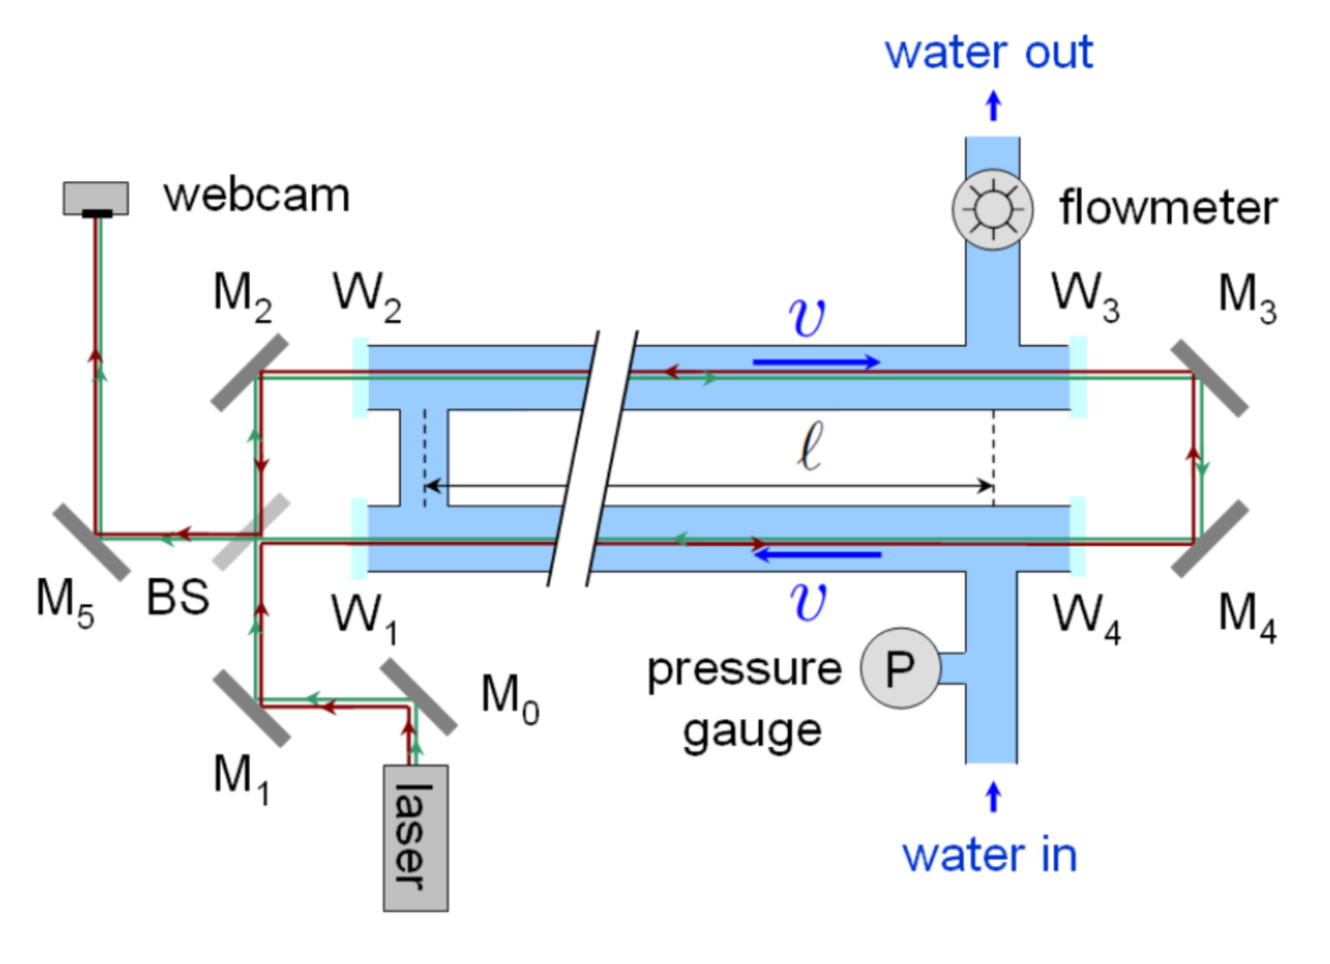
\includegraphics[width=.8\textwidth]{Fizz}
\caption{Fizeau-Experiment}
\label{fizz}
\end{figure}


\chapter{Skript}

\section{Spezielle Relativit"atstheorie}

\[\gamma=\frac{1}{\sqrt{1-\frac{v^2}{c^2}}}\]

Lorenz-Trafo:
\[x'=\gamma(x-ut),\ y'=y,\ z'=z,\ t'=\gamma\left(t-\frac{ux}{c^2}\right)\]

\begin{align*}
v'_x&=\frac{v_x-u}{1-\frac{uv_x}{c^2}}\\
v'_y&=\frac{1}{\gamma}\frac{v_y}{1-\frac{uv_z}{c^2}}\\
v'_z&=\frac{1}{\gamma}\frac{v_z}{1-\frac{uv_x}{c^2}}
\end{align*}

Zeitdilatation:
\[t'=\frac{1}{\gamma}t\]

L"angenkontraktion:
\[l'=\gamma l\]

Doppler:
Klassisch: \[f_B=f_s\frac{c+v_B}{c-v_S}\]
Relativistisch: \[f_B=f_S\frac{\sqrt{1-\frac{v^2}{c^2}}}{1-\cos\alpha\frac{u}{c}}\]

Relativistischer Impuls:
\[\vec{p}=m(v)\vec{v}=\gamma(v)m_0\vec{v}\]

Relativistische Energie-Impuls-Beziehung und Viererimpuls
\[E^2=(m_0c^2)^2+c^2\vec{p}^2\]

\section{Geometrische Optik}

\[n_1\sin\theta_1=n_2\sin\theta_2\]

Lieblingspr"ufungsfrage: Parallel einfallendes Licht, das nicht parallel zur optischen Achse verl"auft, in eine Sammellinse. Strahlen werden immer noch fokussiert aber Brennpunkt verschoben. Konstruktion mit Zentralstrahlengang!

Berechnung Brennpunkt bzw Brennweite
\[\frac{1}{f}=\frac{n_2-n_1}{n_1}\left(\frac{1}{R_1}-\frac{1}{R_2}\right)\]
Brechkraft: \[D=\frac{n}{f}\]

Abbildung \[\frac{1}{f}=\frac{1}{a}+\frac{1}{b}\]

\[\tan\alpha=\mathrm{\frac{Gr"o\ss e des Objkets}{Entfernung des Objekts}}\]
\[V=\mathrm{\frac{Sehwinkel mit Instrment}{Sehwinkel ohne Instrument}}\]
\[L=\mathrm{\frac{Bildgr"o\ss e}{Gegenstandsgr"o\ss e}}\]

Zwei Linsen:
\[\frac{1}{f}=\frac{1}{f_1}+\frac{1}{f_2}\]
\[D_\mathrm{ges}=D_1+D_2\]

Elektronenoptik:\\
Brechindex
\[\frac{n_2}{n_1}=\sqrt{1+\frac{U}{U_0}}\]

\section{Wellenoptik}

Harmonische Ebene 1D Welle:
\[A(x,t)=A_0\cos(\omega t-kx+\vphi)\]

FOURIER TRANSFORMATION

Koh"arenz = Wellen dessen Zeitabh"angigkeiten bis auf Phasendifferenz gleich sind.

Doppelspalt\\
Maxima: \[\sin\alpha=n\frac{\lambda}{d}\]
Minima: \[\sin\alpha=\left(n+\frac{1}{2}\right)\frac{\lambda}{d}\]

Einzelspalt:\\
Intensit"at: \[I(\alpha)=I_0\frac{\sin^2(x)}{x^2}\]
Minima: \[\sin\alpha=n\frac{\lambda}{b}\]
Nebenmaxima: \[\sin\alpha=\left(n+\frac{1}{2}\right)\frac{lambda}{b}\]

Gitter:\\
Intensit"at: \[I(\alpha)=A^2\]
Hauptmaxima: \[\sin\alpha=m\frac{\lambda}{d}\]
Nebenmaxima: \[\sin\alpha=m\frac{\lambda}{Nd}\]
Breite Hauptmaxima: \[B=\frac{2\lambda}{Nd}\]
$\Rightarrow$ scharfe Linien

Bragg:\\
Kristall kann als regelm"a\ss ige Anordnung von Atomen als Raumgitter betrachtet werden:
\[2d\sin\alpha=m\lambda\]

Interferenz an planparallelen Glasplatten:
Just look at the script.

Airy-Formeln:
\begin{align*}
I_R&=I_0\frac{F\sin^2\left(\frac{\Delta\vphi}{2}\right)}{1+F\sin^2\left(\frac{\Delta\vphi}{2}\right)}\\
I_T&=I_0\frac{1}{1+F\sin^2\left(\frac{\Delta\vphi}{2}\right)}
F&=\frac{4R}{(1-R)^2}\\
\frac{\Delta\vphi}{2}&=2\pi\frac{d}{\lambda}\sqrt{n^2-\sin^2\alpha}
\end{align*}

Kirchhoffsches Beugungsintegral
\[\vec{E}(\vec{x}')=\frac{ik}{2\pi}\int Q\tau(x,y)\vec{E}_\mathrm{ein}(\vec{x})\frac{e^{-ikr}}{r}\dd\sigma\]
$Q$ Neigungsfaktor, $\tau$ Transmissionsfunktion (0 oder 1), $r$ Abstand $|\vec{x}-\vec{x}'|$

Beugungsintegral Frauenhofer Beugung:
\[\vec{E}(\vec{x}')=A(\vec{x}')\vec{F}\left(k\frac{x'}{z'},k\frac{y'}{z'}\right)\]

Aufl"osung Lochblende/Linse:
\[\sin\alpha_\mathrm{min}=1.22\frac{\lambda}{D}\]

Aufl"osung Mikroskop:
\[\delta_x\approx0.61\frac{\lambda}{n\sin\vphi}\]

\section{Licht-Materie Wechselwirkung}

% page 46

Transversale welle:
\[\vec{E}\cdot\vec{k}=0\]
Longitudinale Welle:
\[\vec{E}\times\vec{k}=0\]

Lineare Polarisation:
\[\vec{E}=E_0\begin{pmatrix}\cos\tilde{\vphi}\\\sin\tilde{\vphi}\\0\end{pmatrix}\cos(\omega t-kz+\vphi)\]

Zirkulare Polarisation:
\[\vec{E}=E_0\begin{pmatrix}\cos(\omega t-kz+\vphi)\\\pm\sin(\omega t-kz+\vphi)\\0\end{pmatrix}\]
Jede linear polarisierte Welle kann in zwei entgegengesetzte zirkular polarisierte Wellen mit halber Amplitude zerlegt werden und umgekehrt.\\

Elliptische Polarisation:
\[\vec{E}=\begin{pmatrix}E_x\cos(\omega t-kz+\vphi)\\E_y\cos(\omega t-kz+\vphi\pm\frac{\pi}{2})\\0\end{pmatrix}\]

Brechung durch Materie:
\[k_x\neq k_y\]

Stetigkeitsbedingungen:
\[????????????????????????????????????????????????????????????\]

Polarisation eines Dielektrikums:
\[\vec{D}=\vepsilon_0\vec{E}+\vec{P}=\vepsilon_0\vepsilon\vec{E}\]
mikroskopisch ($d$ induziertes Dipolmoment, $\alpha$ Polarisierbarkeit:
\[\vec{d}=\alpha\vec{E}\]

\[\vec{P}=\frac{1}{V}\sum_i\vec{d}_i\]

Wellengleichung in Materie:
\[\Delta\vec{E}-\frac{1}{c_0^2}\frac{\partial^2}{\partial t^2}\frac{\vec{D}}{\vepsilon_0}-\mathrm{grad}\mathop\mathrm{div}\vec{E}=0\]

Komplex:
\[-(k^2)\hat{\vec{E}}_0+\frac{\omega^2}{c_0^2}\hat{\vepsilon}\hat{\vec{E}}_0+(\hat{\vec{k}}\cdot\hat{\vec{E}}_0)\hat{\vec{k}}=0\]
mit:
\[\hat{\vec{k}}^2=\vec{k}'^2-\vec{k}''^2+2i\vec{k}'\cdot\vec{k}''\]

Transversal ($\vec{k}\propto\vec{E}_0$):
\[\hat{\vec{k}}^2=\frac{\omega^2}{c_0^2}\hat{\vepsilon}\]
\[\omega(\hat{\vec{k}})=c_0\sqrt{\frac{\hat{\vec{k}}^2}{\hat{\vepsilon}}}\]

Komplexer Brechungsindex ($K$ Extinktionskoeffizient:
\[\hat{n}=n+iK=\sqrt{\hat{\vepsilon}}\]
\[\sqrt{\hat{\vec{k}}^2}=\frac{\omega}{c_0}\hat{n}\]
Imagin"arer Teil klein $\Rightarrow n=\sqrt{\vepsilon'},\ K=\frac{\vepsilon''}{2n}$

Wirkungsquerschnitt:
\[\frac{\dd^2\sigma}{\dd\Omega\dd E}\]

Rayleigh-Streuung ist $\omega^4$-abh"angig, also werden niedrige Frequenzen (blau) st"arker reflektiert als hohe Frequenzen (rot).

\underline{Zug"angliche Infos im Linienspektrum}
\begin{enumerate}
\item Lage/Frequenz von Peaks gibt Energiedifferenz ("Ubergangsenergie) an:
\[E_2-E_1=kv\]
\item Intensit"at h"angt von "Ubergangswahrscheinlichkeit, Teilchendichte, und St"arke der Wechselwirkungen von Eingestrahlten mit Bestrahlten ab.
\item Linienbreite/-form ist bei Lorenzverteilung mit Lebensdauer verkn"upft:
\[e^{-\nicefrac{t}{\tau}}\]
\end{enumerate}



% page 57















































\end{document}